\documentclass[14pt]{beamer}
\usepackage[T2A]{fontenc}
\usepackage[utf8]{inputenc}
\usepackage[english,bulgarian]{babel}
\usepackage{amssymb,amsfonts,amsmath,mathtext}
\usepackage{cite,enumerate,float,indentfirst}
\usepackage{listings}
\usepackage{animate}
\usepackage{graphicx}
\graphicspath{{images/}}

\usetheme{Pittsburgh}
\usecolortheme{whale}

\setbeamercolor{footline}{fg=blue}
\setbeamertemplate{footline}{
  \leavevmode%
  \hbox{%
  \begin{beamercolorbox}[wd=.333333\paperwidth,ht=2.25ex,dp=1ex,right]{}%
  Стр. \insertframenumber{} от \inserttotalframenumber \hspace*{2ex}
  \end{beamercolorbox}}%
  \vskip0pt%
}

\newcommand{\itemi}{\item[\checkmark]}

\title{\textbf{Обработка на изображения с реакционно-дифузен модел}}
\author{\small{%
\textbf{\emph{Екип:}~Стефан Велинов, Християн Марков, Пламен Никифоров}}\\
\vspace{30pt}%
ПММРП летен семестър 2017\\
ФМИ-СУ%
\vspace{20pt}%
}
\date{\small{София, 2017}}

\begin{document}

\maketitle

\begin{frame}
\frametitle{Основен проблем и подход}
\begin{itemize}
  \item \textbf{Намиране на ръбове, сегментация на изображение, увеличаване на контраста и намаляване на шума}
  \item \textbf{Използване на Тюрингова нестабилност, модел на FitzHugh \& Nagumo, дифузия}
\end{itemize}
\end{frame}

%\begin{frame}
%\frametitle{Цели и задачи}
%\begin{itemize}
%  \item \textbf{Запознаване с процеса на дифузия}
%  \item \textbf{Извеждане на общия вид на уравнение от тип реакция-дифузия}
%  \item \textbf{Запознаване с механизма на Тюринг за генериране на пространствени структури}
%  \item \textbf{Изследване на устойчивост за система ОДУ от първи ред}
%\end{itemize}
%\end{frame}

\begin{frame}
\frametitle{Дифузия}
\begin{itemize}
  \item \textbf{Процес на пренос на субстанция или енергия от област с по-висока концентрация към област с по-ниска концентрация}
  \item \textbf{Всички видове дифузия се подчиняват на едни и същи закони}
  \item \textbf{Закон на Fick:  $ \frac{\partial \varphi}{\partial t} = D \frac{{\partial}^2 u}{\partial x^2} $}
\end{itemize}
\end{frame}

% TO DO: Numerical Euler

\begin{frame}
\frametitle{Числено решаване на дифузия}
\begin{itemize}
  \item \textbf{Метод на Ойлер}
\begin{center}
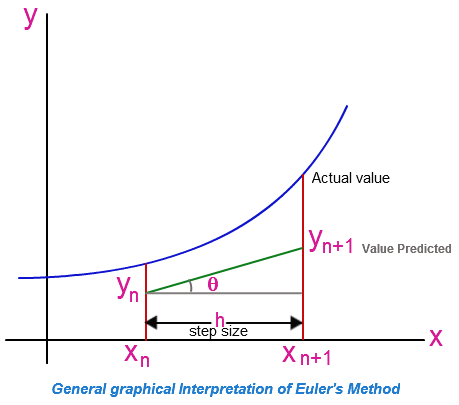
\includegraphics[width=0.5\textwidth]{euler1.png}
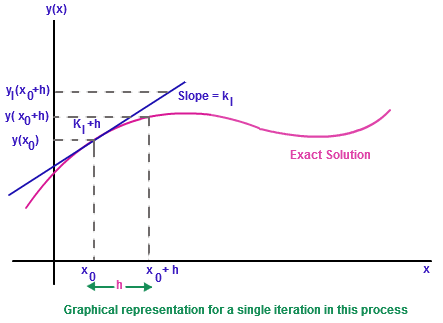
\includegraphics[width=0.5\textwidth]{euler2.png}
\end{center}
\end{itemize}
\end{frame}

\begin{frame}
\frametitle{Дифузията в действие}
\begin{itemize}
  \item Промяна на температурата с течение на времето
\end{itemize}
\begin{center}
%\animategraphics[controls,loop,height=5cm]{5}{./animation/frame_}{0}{123}
\end{center}
\end{frame}

\begin{frame}
\frametitle{Реакция}
\begin{itemize}
  \item \textbf{}
\end{itemize}
\end{frame}

\begin{frame}
\frametitle{Реакция-дифузия}
\begin{itemize}
  \item $\frac{\partial u}{\partial t} = D_{u} \nabla^2 u + \frac{1}{\varepsilon}\cdot u(1-u)(u-a)-v)$\\
  $\frac{\partial v}{\partial t} = D_{v} \nabla^2 v + u -bv$
  \item u и v са концентрациите на активатор и инхибитор
  \item $D_u$ и $D_v$ са коефициенти на дифузия
  \item $(0 < \varepsilon < 1), (0 < a < 0.5), b>0$
\end{itemize}
\end{frame}

%\begin{frame}
%\frametitle{Механизъм на Тюринг}
%\begin{itemize}
%  \item Продуктите на реакцията се разпределят в обема по различен начин: в някои точки са повече, а в други - по-малко
%  \item Редуващите се сгъстявания и разреждания зависят от скоростта на реакцията и скоростта на дифузията
%  \item Подобни модели се използват в изкуството, архитектурата, дизайна
%\end{itemize}
%\end{frame}

\begin{frame}
\frametitle{Устойчивост на ОДУ от първи род}
\begin{itemize}
\item $\frac{\partial u}{\partial x} = f(x,u(x)), x_0 < x \leq X$
\item начално условие $u(x_0) = u_0$
\end{itemize}
\end{frame}

\begin{frame}
\frametitle{Източници}
\begin{itemize}
\item \textbf{M. Ebihara et al., Image Processing by a Discrete Reaction-Diffusion System}
\item \textbf{J. Weickert, Anisotropic Diffusion in Image Processing}
\end{itemize}
\end{frame}

\begin{frame}
\begin{center}
Благодарим за вниманието!
\end{center}
\end{frame}

\end{document}
